% gallery-title: Reduction and injection maps
% gallery-category: Quantum 
% gallery-tags: qubit
% gallery-description: Representation of the action of CPTP projectors
% gallery-order: 10
% paper: arXiv:2412.05102

\documentclass{standalone}

\usepackage{amsfonts,amsmath,amssymb}
\usepackage{cancel}
\usepackage{amsfonts,amsmath,amssymb}
\usepackage[english]{babel}
\usepackage[normalem]{ulem}
\usepackage{hyperref}
\usepackage{amsthm}
\usepackage{graphicx}
\usepackage{xfrac}
\usepackage{subcaption,caption}
\usepackage{epsfig}
\usepackage{ulem}
\usepackage{tikz}
\usepackage{mathrsfs}
\usepackage{bbold}  
\usepackage{soul}
\definecolor{green}{RGB}{90, 190, 105} 
\usepackage{pgfplots}
\usepackage{pgfplotstable} 
\usepgfplotslibrary{groupplots}
\pgfplotsset{compat = newest}

\usepackage{bm}
\usetikzlibrary{shapes,arrows}
\usetikzlibrary{matrix}
\usetikzlibrary{3d}
\usetikzlibrary{calc,patterns,angles,quotes,arrows,automata}
\graphicspath{ {./imgs/}}
\usepackage{tikz-3dplot}

\usepackage{csvsimple}

% ---------------------- Calligrapic
\newcommand{\Ac}{\mathcal{A}}
\newcommand{\Bc}{\mathcal{B}}
\newcommand{\Cc}{\mathcal{C}}
\newcommand{\Dc}{\mathcal{D}}
\newcommand{\Ec}{\mathcal{E}}
\newcommand{\Gc}{\mathcal{G}}
\newcommand{\Oc}{\mathcal{O}}
\newcommand{\Hc}{\mathcal{H}}
\newcommand{\Jc}{\mathcal{J}}
\newcommand{\Rc}{\mathcal{R}}
\newcommand{\Mc}{\mathcal{M}}
\newcommand{\Sc}{\mathcal{S}}
\newcommand{\Pc}{\mathcal{P}}
\newcommand{\Zc}{\mathcal{Z}}
\newcommand{\Qc}{\mathcal{Q}}
\newcommand{\Ic}{\mathcal{I}}
\newcommand{\Kc}{\mathcal{K}}
\newcommand{\Lc}{\mathcal{L}}
\newcommand{\Tc}{\mathcal{T}}

% -------------------------- Script
\newcommand{\As}{\mathscr{A}}
\newcommand{\Bs}{\mathscr{B}}
\newcommand{\Cs}{\mathscr{C}}
\newcommand{\Ds}{\mathscr{D}}
\newcommand{\Ls}{\mathscr{L}}
\newcommand{\Os}{\mathscr{O}}
\newcommand{\Ss}{\mathscr{S}}
\newcommand{\Ns}{\mathscr{N}}
\newcommand{\Vs}{\mathscr{V}}
\newcommand{\Ws}{\mathscr{W}}
\newcommand{\Xs}{\mathscr{X}}
\newcommand{\Ys}{\mathscr{Y}}
\newcommand{\Zs}{\mathscr{Z}}

\newcommand{\Rs}{\mathscr{R}}
\newcommand{\Es}{\mathscr{E}}
\newcommand{\Ts}{\mathscr{T}}
\newcommand{\Us}{\mathscr{U}}
\newcommand{\Gs}{\mathscr{G}}
\newcommand{\Fs}{\mathscr{F}}

% -------------------------- Bold
\newcommand{\Rb}{\mathbb{R}}
\newcommand{\Nb}{\mathbb{N}}
\newcommand{\Cb}{\mathbb{C}}
\newcommand{\Pb}{\mathbb{P}}
\newcommand{\Eb}{\mathbb{E}}
\newcommand{\Jb}{\mathbb{J}}

% ------------------------- Fraktur
\newcommand{\Bf}{\mathfrak{B}}
\newcommand{\Ff}{\mathfrak{F}}
\newcommand{\Hf}{\mathfrak{H}}
\newcommand{\Df}{\mathfrak{D}}
\newcommand{\Gf}{\mathfrak{G}}
\newcommand{\Sf}{\mathfrak{S}}
\newcommand{\Zf}{\mathfrak{Z}}
\newcommand{\Pf}{\mathfrak{P}}
\newcommand{\Kf}{\mathfrak{K}}


% -------------------------- Conditional expectations etc
\newcommand{\CE}{\mathbb{E}|}
\newcommand{\SR}{\mathbb{S}|}
\newcommand{\SE}{\mathbb{J}|}

\newcommand{\cov}{{\mathbb{Cov}}}
\newcommand{\var}{{\mathbb{Var}}}

% -------------------------- Reduced operators 
\newcommand{\ro}{\mathcal{R}_0}
\newcommand{\eo}{\mathcal{J}_0}
\newcommand{\rs}{\mathcal{R}}
\newcommand{\es}{\mathcal{J}}

% ------------------------ Numbers
\newcommand{\um}{\frac{1}{2}}
\newcommand{\one}{\mathbb{1}}
\newcommand{\zero}{\mathbb{0}}

\newcommand{\onev}{{\bm 1}}
\newcommand{\zerov}{{\bm 0}}

% ----------------------- Functions and operations
\newcommand{\im}{{\rm Im}}
\newcommand{\id}{{\rm Id}}
\newcommand{\fix}{{\rm fix}}
\newcommand{\ad}{{\rm ad}}
\newcommand{\bin}{{\rm bin}}
\newcommand{\tr}{{\rm tr}}
\newcommand{\diag}{{\rm diag}}
\newcommand{\Span}{{\rm span}}
\newcommand{\cl}{{\rm cl}}
\newcommand{\spec}{{\rm spec}}
\newcommand{\idem}{ {\rm idem}}
\newcommand{\res}{{\rm res}}
\newcommand{\supp}{{\rm supp}}
\newcommand{\lind}{\mathcal{L}}
\newcommand{\alg}{{\rm alg}}
\newcommand{\img}{{\rm Im}}

\DeclareMathOperator{\rank}{rank}

\newcommand{\comp}{{\sim}}
\newcommand{\zentrum}{\mathcal{Z}}


% -------------------------- Inner products and co
\newcommand{\ket}[1]{\left| #1 \right>}
\newcommand{\bra}[1]{\left< #1 \right|}
\newcommand{\norm}[1]{\left|\left| #1 \right|\right|}
\newcommand{\inner}[2]{\left< #1,#2 \right>}
\newcommand{\Outer}[2]{ \left|#1\right>\left<#2\right| }
\newcommand{\expect}[1]{\left< #1 \right>}
\newcommand{\braket}[2]{\left< #1 \middle\vert #2 \right>}
\newcommand{\ketbra}[2]{\left\vert #1 \middle>\middle< #2 \right\vert}
\newcommand{\virg}[1]{\lq\lq{} #1\ignorespacesafterend\rq\rq}

% \usepackage{mathabx}
% \renewcommand{\check}{\widecheck}
% \renewcommand{\bar}{\overline}
% \renewcommand{\Tilde}{\widetilde}
% \renewcommand{\Hat}{\widehat}



% ------------------------ Comments
\newcommand{\blue}[1]{{\color{blue} #1}}
\newcommand{\red}[1]{{\color{red} #1}}
\newcommand{\green}{\color{teal}}

\definecolor{darkviolet}{rgb}{0.58, 0.0, 0.83}
\definecolor{lavender}{rgb}{0.45, 0.31, 0.59}

\newcommand{\TG}[1]{{\color{OrangeRed}#1}}

\newcommand{\LV}[1]{{\color{cyan}#1}}
%{{\color{darkviolet}#1}}
\newcommand{\VL}[1]{{\color{blue}#1}}

\newcommand{\FT}[1]{{\color{ForestGreen}#1}}
\newcommand{\DT}[1]{{\color{Mulberry}#1}}


\usetikzlibrary{positioning}

\begin{document}

    \centering
    \begin{tikzpicture}[align=center, node distance = 3cm]
    \node[] (O) {$\simeq$};
    \node[below right = -0.3cm of O]{
    \begin{tikzpicture}[scale=0.5, every node/.style={scale=0.6}]
        \draw[step=.5cm,gray!50,very thin] (0,0) grid (4.5,4.5);
        \fill [fill=red!50, draw=red, very thick, opacity = 0.5]     (0,2.5) -- (0,4.5) -- (2,4.5) -- (2,2.5) -- cycle;
        \fill [fill=orange!50!white, draw=orange, very thick , opacity = 0.5]     (2,1.5) -- (2,2.5) -- (3,2.5) -- (3,1.5) -- cycle;
        \fill [fill=green!50!white, draw=green, very thick, , opacity = 0.5]     (3,0) -- (3,1.5) -- (4.5,1.5) -- (4.5,0) -- cycle;
        \draw (0.7,3.8) node {$A$};
        \draw (2.2,2.3) node {$B$};
        \draw (3.45,1.05) node {$C$};
    \end{tikzpicture}
    };
    \node[above left = -0.4cm of O]{
    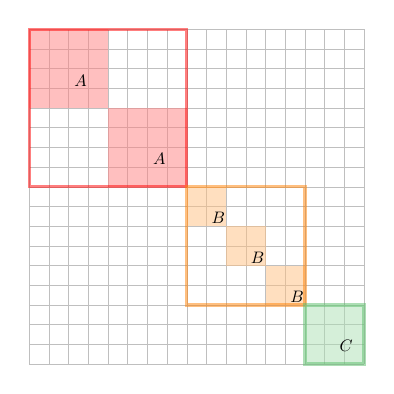
\begin{tikzpicture}[scale=0.5, every node/.style={scale=0.6}]
        \draw[step=.5cm,gray!50,very thin] (0,0) grid (8.5,8.5);
        \fill [fill=red!50!white, opacity = 0.5]     (2,4.5) -- (2,6.5) -- (4,6.5) -- (4,4.5) -- cycle;
        \fill [fill=red!50!white, opacity = 0.5]     (0,6.5) -- (0,8.5) -- (2,8.5) -- (2,6.5) -- cycle;
        \fill [fill=none, draw=red, very thick, opacity = 0.5]     (0,4.5) -- (0,8.5) -- (4,8.5) -- (4,4.5) -- cycle;
        \fill [fill=orange!50!white, opacity = 0.5]     (4,3.5) -- (4,4.5) -- (5,4.5) -- (5,3.5) -- cycle;
        \fill [fill=orange!50!white, opacity = 0.5]     (5,2.5) -- (5,3.5) -- (6,3.5) -- (6,2.5) -- cycle;
        \fill [fill=orange!50!white, opacity = 0.5]     (6,1.5) -- (6,2.5) -- (7,2.5) -- (7,1.5) -- cycle;
        \fill [fill=none, draw=orange, very thick, opacity = 0.5]     (4,1.5) -- (4,4.5) -- (7,4.5) -- (7,1.5) -- cycle;
        \fill [fill=green!50!white, draw=green, very thick, opacity = 0.5]     (7,0) -- (7,1.5) -- (8.5,1.5) -- (8.5,0) -- cycle;
        \draw (1.3,7.2) node {$A$};
        \draw (3.3,5.2) node {$A$};
        \draw (4.8,3.7) node {$B$};
        \draw (5.8,2.7) node {$B$};
        \draw (6.8,1.7) node {$B$};
        \draw (8.05,0.45) node {$C$};
    \end{tikzpicture}
    };

\draw (0,3) node (C) {};  
\draw (2,0) node (D) {};  
\draw[-stealth, thick] (C) to [bend left=35] (D);

\draw (-3,0) node (E) {};  
\draw (0,-2) node (F) {};  
\draw[-stealth, thick] (F) to [bend left=35] (E);

\draw (1.8,1.8) node[label={$\Rc$}] (C) {};
\draw (-2.2,-2.2) node[label={$\Jc$}] (C) {};
    
    \end{tikzpicture}
\end{document}